\chapter{Deep Equilibrium Models}
\label{chapter:deep_equilibrium_models}

\section{Steady State Problems}
\label{sec:steady_state_problems}

Steady State Problems involve determining the equilibrium state of a system, i.e., the state of the system where the rate of change of the system is zero. Let, our steady state problem be defined as follows:
%
\begin{equation}
  \frac{\partial z}{\partial t} = \func{f_\theta}{z, t} - z
\end{equation}
%
In case of continuous dynamical systems, the steady state would be determined by the partial derivative w.r.t. time being zero:
%
\begin{equation}
  \frac{\partial z}{\partial t} = 0
\end{equation}
%
In case of discrete dynamical systems, the steady state would be defined by states remaining constant over time:
%
\begin{equation}
  z_{n + 1} = z_n \implies \zstar = \func{f_\theta}{\zstar, \infty}
\end{equation}
%
There are two ways to solve steady state problems:
%
\begin{enumerate}
  \item \textbf{Treating it as a Nonlinear Problem}: \todo{}
  \item \textbf{Treating it as an ODE with custom termination criteria}: \todo{}
\end{enumerate}
%

\todo{\url{https://docs.sciml.ai/NonlinearSolve/stable/solvers/SteadyStateSolvers/}}

\section{Sensitivity Analysis of Steady State Problems}
\label{sec:sensitivity_analysis_ssproblems}

Let, $\zstar$ be the steady state solution of the system, i.e., $\zstar = \func{f_\theta}{\zstar, \infty}$. For the sake of brevity, let us drop the $t = \infty$ term, i.e., $\zstar = \func{f_\theta}{\zstar}$. Differentiating w.r.t. $\theta$ we get:
%
\begin{align}
           & \frac{\partial \zstar}{\partial \theta} = \frac{\partial \func{f_\theta}{\zstar}}{\partial \zstar} \times \frac{\partial \zstar}{\partial \theta} + \frac{\partial \func{f_\theta}{\zstar}}{\partial \theta}\\
  \implies & \left( I - \frac{\partial \func{f_\theta}{\zstar}}{\partial \zstar} \right) \times \frac{\partial \zstar}{\partial \theta} = \frac{\partial \func{f_\theta}{\zstar}}{\partial \theta}\\
\end{align}
%
Let, the cost function we are optimizing be $\func{g}{\zstar, \theta}$. We have:
%
\begin{align}
  \frac{d \func{g}{\zstar, \theta}}{d \theta} &= \frac{\partial \func{g}{\zstar, \theta}}{\partial \zstar} \times \frac{\partial \zstar}{\partial \theta} + \frac{\partial \func{g}{\zstar, \theta}}{\partial \theta}\\
  &= \frac{\partial \func{g}{\zstar, \theta}}{\partial \zstar} \times \left( I - \frac{\partial \func{f_\theta}{\zstar}}{\partial \zstar} \right)^{-1} \times \frac{\partial \func{f_\theta}{\zstar}}{\partial \theta} + \frac{\partial \func{g}{\zstar, \theta}}{\partial \theta} \label{eq:ss_gradient}
\end{align}
%
Let, the size of the parameters be $L_\theta$ and the size of the states be $L_z$. The RHS of the above equation involves:
%
\begin{enumerate}
  \item $\frac{\partial \func{g}{\zstar, \theta}}{\partial \theta}$: $1 \times L_\theta$ matrix
  \item $\frac{\partial \func{g}{\zstar, \theta}}{\partial \zstar}$: $1 \times L_z$ matrix
  \item $\left( I - \frac{\partial \func{f_\theta}{\zstar}}{\partial \zstar} \right)^{-1}$: $L_z \times L_z$ matrix
  \item $\frac{\partial \func{f_\theta}{\zstar}}{\partial \theta}$: $L_z \times L_\theta$ matrix
\end{enumerate}
%
Instead of directly computing the RHS, we can solve a linear system of equations for $\lambda$:
%
\begin{equation}
  \left( I - \frac{\partial \func{f_\theta}{\zstar}}{\partial \zstar} \right)^T \times \lambda = \left(\frac{\partial \func{g}{\zstar, \theta}}{\partial \zstar}\right)^T
\end{equation}
%
Substituting $\lambda^T$ in the \cref{eq:ss_gradient}, we get:
%
\begin{equation}
  \frac{d \func{g}{\zstar, \theta}}{d \theta} = \lambda^T \times \frac{\partial \func{f_\theta}{\zstar}}{\partial \theta} + \frac{\partial \func{g}{\zstar, \theta}}{\partial \theta}
\end{equation}
%
Hence, sensitivity analysis of a steady state problem boils down to solving a linear system of equations and a matrix-vector product.


\section{Deep Equilibrium Networks}
\label{sec:deep_equilibrium_networks}

\begin{figure}[h]
  \centering
  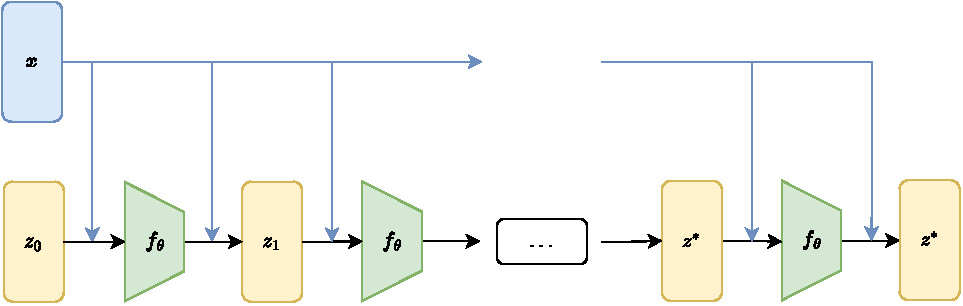
\includegraphics[width=0.9\textwidth]{../figures/deep_equilibrium_models/model_architecture.pdf}
  \caption{\textbf{Discrete DEQ Formulation}: Discrete DEQ Block where the input $x$ is injected at every iteration till the system (with initial state $z_0$) converges to a steady $\zstar$.}
  \label{fig:model_architecture_discrete_deq}
\end{figure}

Deep Equilibrium Networks (DEQs)~\citep{bai_deep_2019} are implicit models where the output space represents a steady-state solution. Intuitively, this represents infinitely deep neural networks with input injection, i.e., an infinite composition of explicit layers $z_{n + 1} = f_\theta(z_n, x)$ with $z_0 = 0$ and $n \rightarrow \infty$. In practice, it is equivalent to evaluating a dynamical system until it reaches a steady state $\zstar = f_\theta(\zstar, x)$.

% \citet{bai_deep_2019, bai_multiscale_2020} perform nonlinear fixed point iterations of the discrete dynamical system using Broyden's method~\citep{broyden1965class, bai_multiscale_2020} to reach this steady-state solution. 

Evaluating DEQs requires solving a steady-state equation involving multiple evaluations of the explicit layer slowing down the forward pass. However, driving the solution to steady-state makes the backward pass very efficient~\citep{johnson2012notes} (See \Cref{sec:sensitivity_analysis_ssproblems}). Despite a potentially infinite number of evaluations of $f_\theta$ in the forward pass, backpropagation only requires solving a linear equation.

\subsection{Nonlinear Solvers}
\label{ssec:nonlinear_solvers_deqs}


\subsection{Adjoint Equations}
\label{subsec:adjoint_equations_deqs}

\subsection{Newton-Krylov Methods for solving Linear Systems}
\label{subsec:newton_krylov_methods}

\section{Convergence Criteria}
\label{sec:ssproblem_convergence_criteria}

\todo{\url{https://docs.sciml.ai/NonlinearSolve/stable/basics/TerminationCondition/}}

\section{Common Applications of DEQs}
\label{sec:common_applications_deqs}

\section{Accelerating DEQs}
\label{sec:accelerating_deqs}

